\section*{Aufgabe 6}

Welche der folgenden prädikatenlogischen Formeln (über einem nicht leeren Gültigkeitsbereich für die Variable x) stellen allgemeingültige Aussagen dar, welche nicht:

\begin{enumerate}[label={a)}, leftmargin=*]
\item $(\forall x : F(x)) \Rightarrow (\lnot \forall x : \lnot F(x))$
\end{enumerate}

\textit{Richtig, da $\lnot \forall x : \lnot F(x)$ sich als $\exists x : F(x)$ schreiben lässt, und $\forall x : F(x))$, $\exists x : F(x)$ impliziert.}

\begin{enumerate}[label={b)}, leftmargin=*]
\item $(\forall x : F(x) \land G(x)) \Rightarrow (\forall x : G(x))$
\end{enumerate}

\textit{Richtig.}\\

\begin{table}[h]
\centering
\begin{tabular}{c|c|c|c}
$F(x)$ & $G(x)$ & $\overbrace{F(x) \land G(x)}^{H}$ & $H \Rightarrow G(x)$\\
0 & 0 & 0 & 1\\
1 & 1 & 1 & 1
\end{tabular}
\end{table}\

\begin{enumerate}[label={c)}, leftmargin=*]
\item $(\forall x : F(x) \lor G(x)) \Rightarrow (\forall x : F(x))$
\end{enumerate}

\textit{Falsch. Bei der Belegung $0$, $0$ entsteht ein Widerspruch zur Aussage.}

\begin{table}[h]
\centering
\begin{tabular}{c|c|c|c}
$F(x)$ & $G(x)$ & $\overbrace{F(x) \land G(x)}^{H}$ & $H \Rightarrow G(x)$\\
0 & 0 & 0 & 1\\
\end{tabular}
\end{table}\

\begin{enumerate}[label={d)}, leftmargin=*]
\item $(\forall x : F(x) \lor G(x)) \Rightarrow (\exists x : G(x))$
\end{enumerate}

\textit{Falsch. Beispiel: Sei F(x) $x^2 \geq 0$ und G(x) sei $x < 0$ für $x \in \mathbb{R}$, so gilt zwar $\forall x : F(x) \lor G(x)$ aber nicht $\exists x : G(x)$.}

\newpage

\begin{enumerate}[label={e)}, leftmargin=*]
\item $(\forall x : F(x) \Rightarrow G(x)) \Rightarrow (\exists x : F(x) \land G(x))$
\end{enumerate}

\textit{Falsch. Erklärung durch Venn-Diagram: Sei F(x), dass ein Element in F enthalten ist und G(x), dass ein Element in G enthalten ist, dann bedeutet $\forall x : F(x) \Rightarrow G(x)$, dass gilt, dass alle Elemente die in F enthalten sind auch in G enthalten sind. Daraus folgt allerdings nicht, dass es mindestens ein Element gibt welches in F und G enthalten ist, da, da es auch ein Element geben kann welche nur in G enthalten ist aber nicht in F.}

\begin{center}
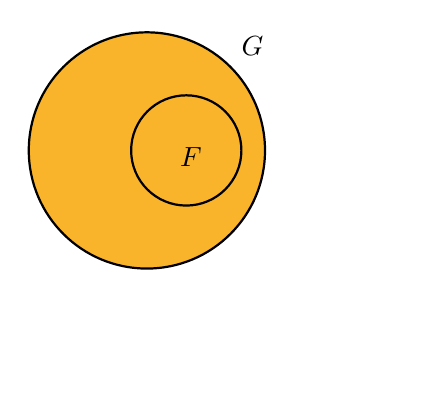
\begin{tikzpicture}[thick,
    set/.style = {circle,
        minimum size = 3cm}]
 
% Set G
\node[set,label={45:$G$}, fill=Dandelion] (G) at (0,0) {};
 
% Circles outline
\draw (0,0) circle(1.5cm);
\draw (0.5,0) circle(0.7cm);

% Set F
\node[set,label={135:$F$}] (F) at (1.9,-1.4) {};

\end{tikzpicture}
\end{center}